\documentclass[a4paper,12pt]{article}

\usepackage{tikz}		
\usepackage{url}
\usepackage{amsmath}
\usepackage{graphicx}
\usepackage{pgfplots}
\usepackage{listings}
\usepackage{hyperref}
\usepackage[czech]{babel}

\author{Moravec Vojtěch}
\title{Analýza sítě odpovědí na stránce \emph{MathOverflow}}
\date{Zimní semestr 2018}

\begin{document}

\maketitle
\newpage

\section{Popis datasetu}

Analyzovaný dataset byl získán ze stránky \emph{snap.stanford.edu} \cite{snapnets}. Dataset obsahuje
seznam hran orientované grafu, který reprezentuje interakci mezi uživateli stránky
 \emph{https://mathoverflow.net/}. Hrana ($u$,$v$) vycházející z vrcholu $v$ do vrcholu $u$, znamená, že
 uživatel $u$ odpověděl na otázku uživatele $v$. Originální dataset obsahuje také časové razítka vzniku
 hrany, ale pro naše účely je budeme ignorovat a budeme pracovat se všemi hranami.
 
\section{Analýza sítě}
Síť obsahuje $21 688$ vrcholů a $107 581$ hran, tedy mezi $21 668$ uživateli bylo 
zodpovězeno $107 581$ otázek.

\begin{table}[h!]
\centering
\begin{tabular}{l | r | r | r | r | r}
 				& Minimum & Výskyt	& Maximum & Výskyt	& Průměr \\
\hline
Vstupní stupeň 	& 0 & $5683 \times$	& 1102 	& 	$1 \times$	& 4,9604 \\
Výstupní stupeň & 0 & $11309 \times$& 1415 	& 	$1 \times$	& 4,9603 \\
Celkový stupeň  & 1	& $9445 \times$	& 1815	&	$1 \times$	& 9,9207
\end{tabular}
\caption{Tabulka stupňů vrcholů}
\label{tab:degree}
\end{table}

Z Tabulky \ref{tab:degree} můžeme vyčíst, tyto extrémy:
\begin{itemize}
\item 5683 uživatelům nepřišla žádná odpověď.
\item Jednomu uživateli přišlo celkem 1102 odpovědí na jeho otázky.
\item 11309 uživatelů neodpovědělo na žádnou otázku.
\item Nejvíce odpovědí napsal jeden uživatel a to 1415 odpovědí.
\end{itemize}

Průměrný uživatel napsal skoro 5 odpovědí na otázky ostatních a taktéž průměrně získal 5 odpovědí 
od ostatních uživatelů.

Dále na Obrázcích \ref{img:in_deg_rel} a \ref{img:out_deg_rel} můžeme v grafech vidět relativní
distribuci stupňů. Tato distribuce odpovídá mocninnému dělení, jak je tomu u obecně u reálných sítí.

\begin{figure}[h!]
\centering
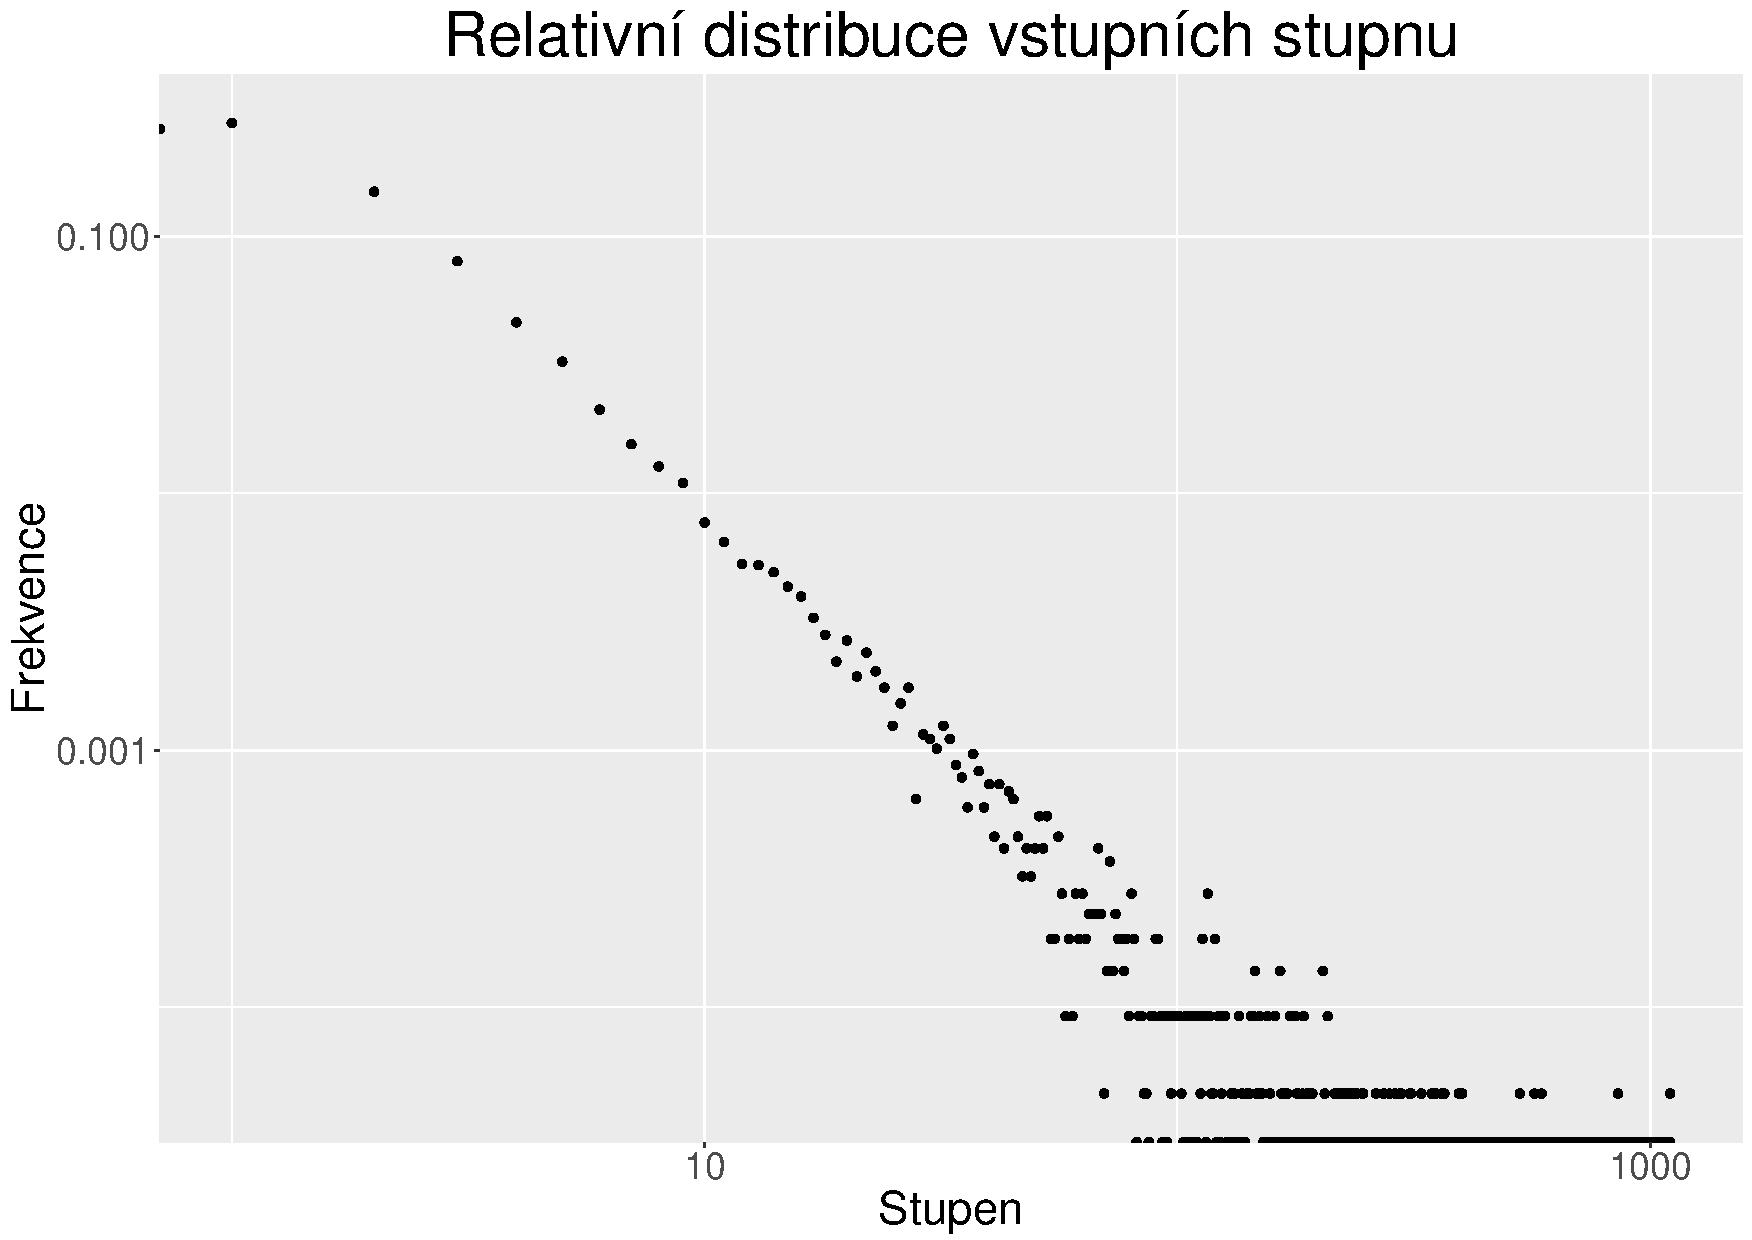
\includegraphics[scale=0.4]{images/in_deg_rel.pdf}
\caption{Graf relativní distribuce vstupních stupňů}
\label{img:in_deg_rel}
\end{figure}

\begin{figure}[h!]
\centering
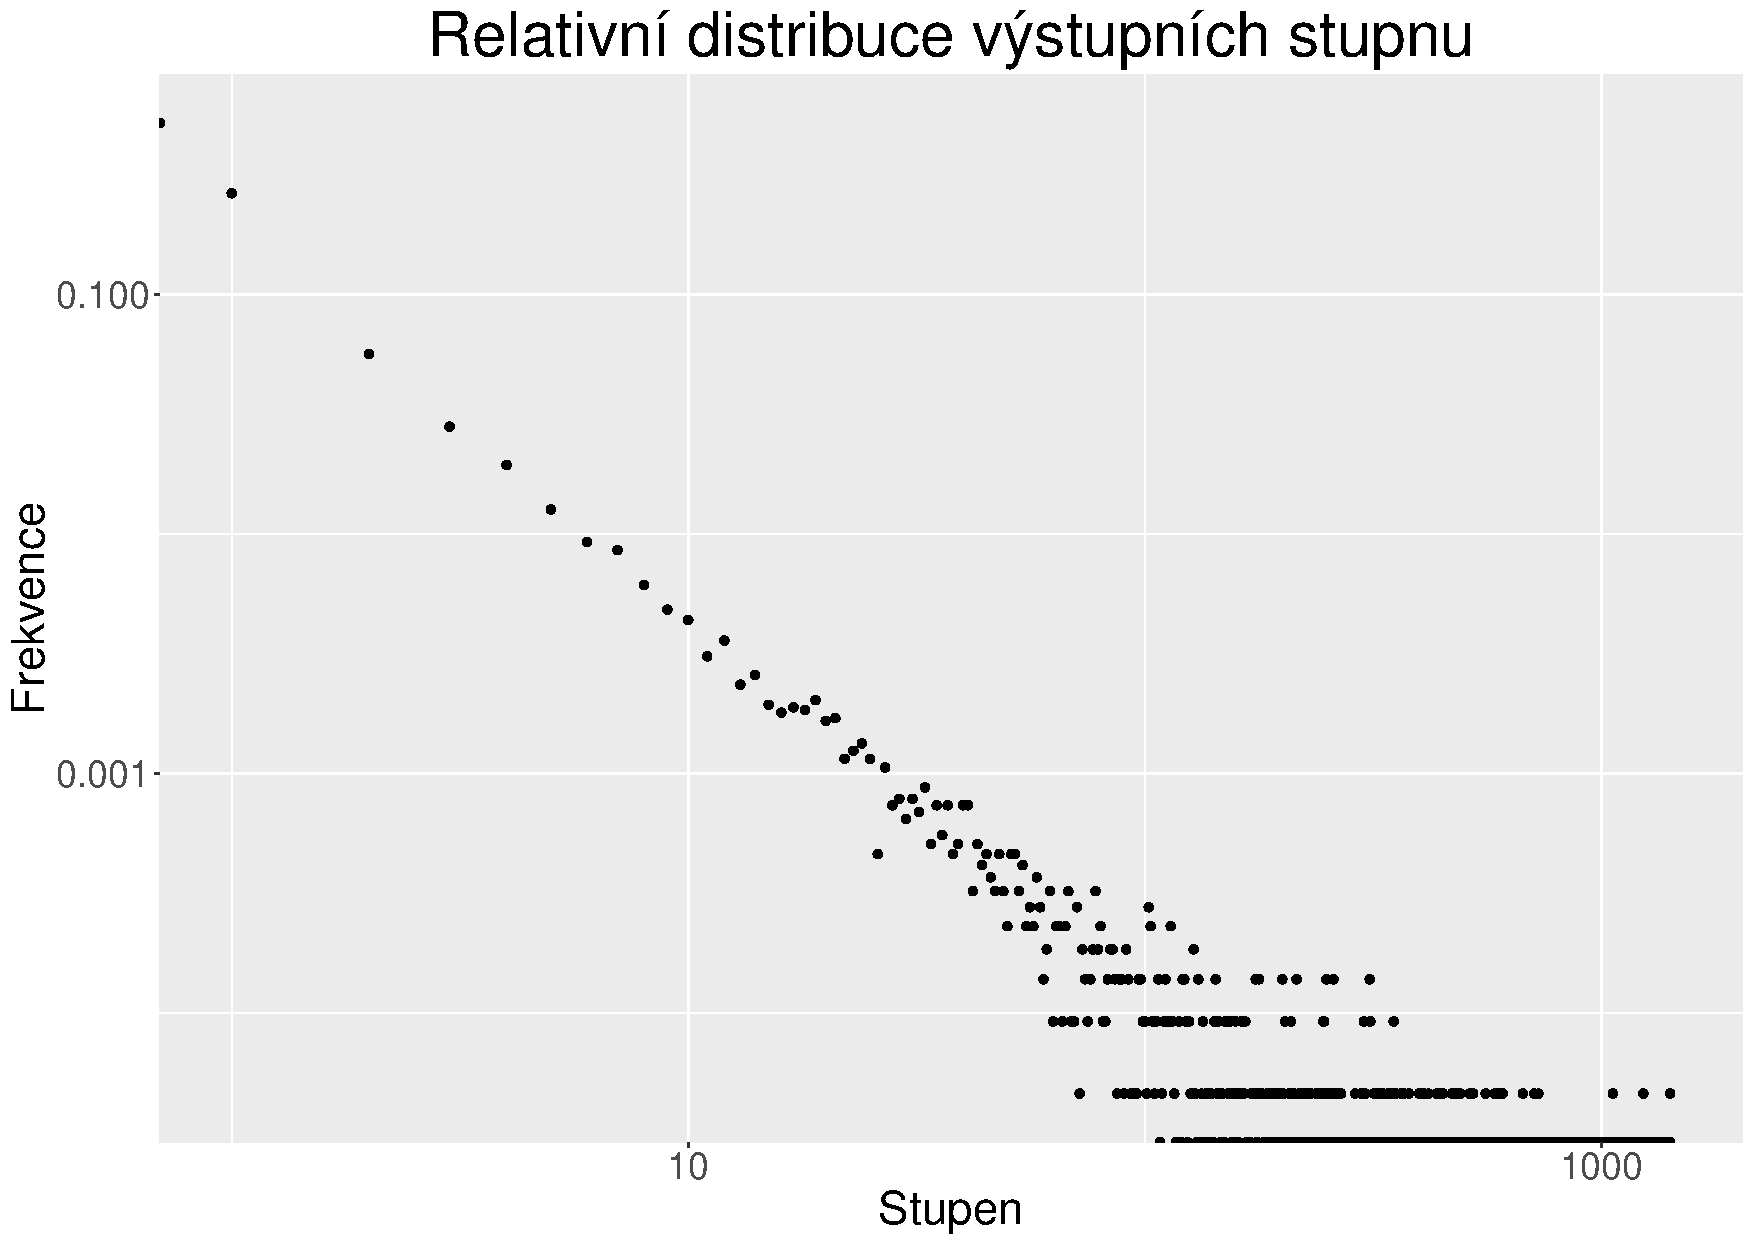
\includegraphics[scale=0.4]{images/out_deg_rel.pdf}
\caption{Graf relativní distribuce výstupních stupňů}
\label{img:out_deg_rel}
\end{figure}



\bibliography{citations}
\bibliographystyle{ieeetr}

\end{document}